%!TEX root = ../thesis.tex
Before continuing on the topic of jamming interfaces, let us first give an introduction to the mechanics of jamming.

Jamming is a mechanism that can enable granular material to transition between solid-like and liquid-like states. 
These states are achieved by varying an external stress on the material.
Even though a granular material is not a compound in itself these states show that it resembles the behaviour of a chemical compound such as water, which can shift between vapor, liquid and ice under an external stress such as temperature.
A granular material, such as sand may resemble a liquid as it flows through an hour glass, although the individual grains themselves are a solid structure. 
If this granular material exist within a confined space and are put under an external stress such as pressure, they jam against each other with no ability to escape.
Figure~\ref{fig:ch:jamming:particles:jam_unjam} illustrates the behaviour of granular material in the two states.

\begin{figure}[h]
\centering
\begin{subfigure}[b]{.44\textwidth}
  \centering
  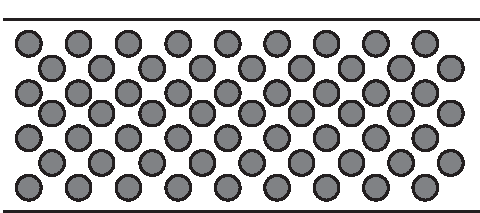
\includegraphics[width=\linewidth]{figures/jamming/particles_unjammed.pdf}
  \caption{Granular material flowing freely in a liquid-like state.}
\end{subfigure}%
\hspace{0.02\textwidth}
\begin{subfigure}[b]{.44\textwidth}
  \centering
  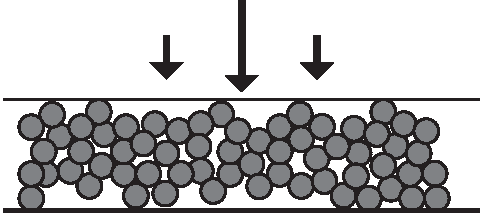
\includegraphics[width=\linewidth]{figures/jamming/particles_jammed.pdf}
  \caption{Granular material jammed in a confined space due to pressure.}
\end{subfigure}
\caption{Different granular material.}
\label{fig:ch:jamming:particles:jam_unjam}
\end{figure}

You might have noticed how some coffee packagings at the local super market are like a rigid container, see figure~\ref{fig:ch:jamming:coffee-packaging}. 
In this kind of packaging, after filling it with coffee, all excess air has been sucked out by applying a vacuum, thereby jamming the coffee grains and making it almost rock solid. 
After opening the packaging the form and viscosity of the structure change instantly as air is let in releasing coffee grains from their jammed state.
Another example is a regular bean bag which exhibits some of the same properties, see figure~\ref{fig:ch:jamming:bean-bag}. 
When no force is applied to it, i.e. no one is sitting in it, it resembles the liquid-like state mentioned earlier. 
Then, when a person sits down in it, air will be pressed out and the particles (most often polystyrene foam) will be pushed tightly together filling voids and thereby jamming the particles making it resemble a solid.

\begin{figure}[h]
\centering
\begin{minipage}[t]{.44\textwidth}
  \centering
  \includegraphics[width=.5\linewidth]{figures/jamming/coffee_packaging}
  \captionof{figure}{Coffee in vacuum packaging.}
  \label{fig:ch:jamming:coffee-packaging}
\end{minipage}%
\hspace{0.02\textwidth}
\begin{minipage}[t]{.44\textwidth}
  \centering
  \includegraphics[width=.5\linewidth]{figures/jamming/bean_bag}
  \captionof{figure}{A bean bag.}
  \label{fig:ch:jamming:bean-bag}
\end{minipage}
\end{figure}

\subsection{Particles}
\label{ch:jamming:particles}
The granular material, also called the particles, can be any material that has the physical properties that allow for jamming to occur. 
But parameters such as particle size, shape and compressibility have an impact on the jamming transition. 
This has been investigated by several researchers, e.g. \cite{cheng2012design} and \cite{steltz2010jamming}, where the stress to strain ratio of different granular materials are evaluated. 
Ground coffee (fine and coarse) and glass beads of varying size are recurring across these tests, the first being an irregular shape with a rough surface as opposed to the plain shape and smooth surface of the second, see figure~\ref{fig:ch:jamming:particles-close-up}. 
Particles of same size and with a smooth surface will tend to be more fluid-like when unjammed as they flow more freely. 
Irregular particles with rough surfaces will create more friction between the particles thus being less fluid-like in the unjammed state.
Furthermore, the bigger the particles the more influence on the surface structure of the container they will have in terms of surface texture.

The conclusion is that the choice of granular material is very much dependent on the application in question. 

\begin{figure}
\centering
\begin{subfigure}{.44\textwidth}
  \centering
  \includegraphics[width=\linewidth]{figures/jamming/coffee-grains}
  \caption{Ground coffee}
\end{subfigure}%
\hspace{0.02\textwidth}
\begin{subfigure}{.44\textwidth}
  \centering
  \includegraphics[width=\linewidth]{figures/jamming/glass-beads}
  \caption{Glass beads}
\end{subfigure}
\caption{Different granular material.}
\label{fig:ch:jamming:particles-close-up}
\end{figure}

%\todo{research in particle parameters in other\\ disciplines such as robotics.}

%\begin{itemize}
%	\item http://en.wikipedia.org/wiki/Jamming\_(physics)
%	\item http://www.nature.com/nphys/journal/v3/n4/full/nphys580.html
%	\item http://www.nature.com/nature/journal/v411/n6839/full/411772a0.html
%\end{itemize}

\subsection{The technique}
\label{ch:jamming:technique}

The jamming technique can be applied with both a pneumatic and a hydraulic approach.
In the pneumatic approach a gas, for example air, is used as a means for actuation, see figure~\ref{fig:ch:jamming:jamming-basics}.
The gas is enclosed together with granular material within a flexible and air tight container, for example rubber latex. 
A filter prevents the granular material from escaping the container and a valve upholds the pressure.
An external vacuum pump can then suck out the air of the container, creating a negative pressure inside, which results in the transition to a solid-like form. 
The speed of this transition of course depends on the suction power of the pump.
When the vacuum is released the form will gradually transition back to the liquid state. 
In this way, the transition allows for states in between the two extremes; solid and liquid.
By sensing and adjusting the pressure inside a jamming volume the stiffness can be controlled and thereby be in any intermediate state in between solid and liquid giving complete control of the viscosity of the volume.
Changing the stiffness of a volume by jamming also affects other types of shape-change than viscosity.
Viscosity change affects the bearing ability of the volume which in turns has an effect on the form, like in the previous coffee bag example.
Additionally, when approaching maximum stiffness the inner particles can begin to appear on the surface and thereby affect the texture of the object.
\begin{figure}[h]
  \centering
  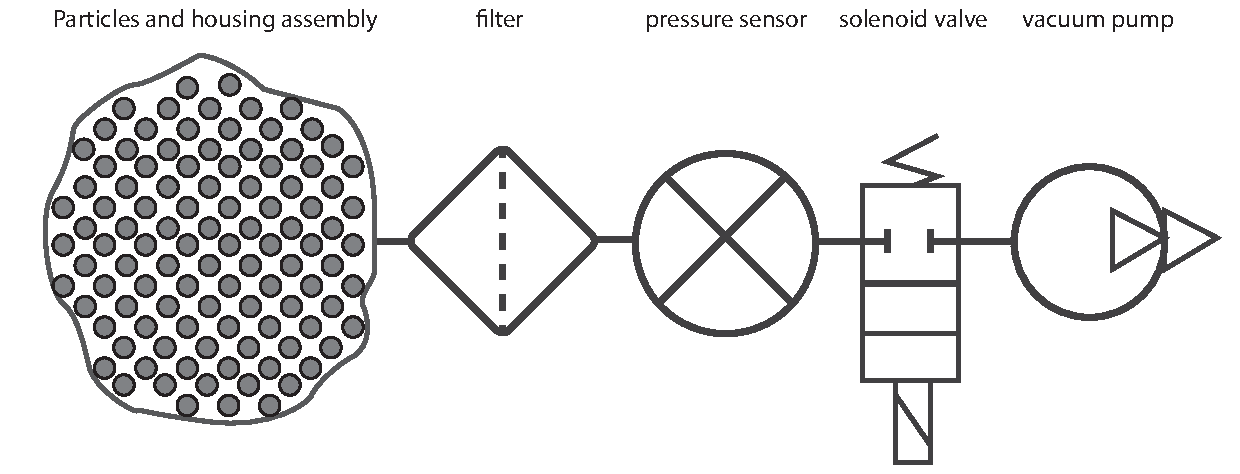
\includegraphics[width=.9\textwidth]{figures/jamming/jamming-basics.pdf}
  \caption{A basic pneumatic jamming system.}
  \label{fig:ch:jamming:jamming-basics}
\end{figure}

Jamming makes it possible to deform an object by hand while in the liquid state and then apply the vacuum and make the deformed object solid - in a sense the form is \emph{saved} as long as the vacuum is maintained.
Figure~\ref{fig:ch:jamming:jamming-transition} shows a transition where a form has been molded and solidified into a shape.
When the pressure is released the form gradually changes shape as seen in the individual steps of the figure.
In this setup we used a balloon as the membrane and ground coffee within as particles.
Pressure was applied with a vacuum cleaner and a coffee filter prevents the particles from being sucked out.
In the example it can be seen that the object (balloon) returns to its initial state which is a requirement for SCIs as stated earlier in section \ref{ch:jamming:vocabulary}.
In this example it is the tension of the rubber latex of the balloon that forces it back but it could as well have been an actuation done with the jamming technique itself. 

\begin{figure}[h]
  \centering
  \includegraphics[width=.9\textwidth]{figures/jamming/jamming-transition}
  \caption[A jamming transition setup.]
  {Jamming transition with a balloon, ground coffee, vacuum cleaner and a coffee filter.}
  \label{fig:ch:jamming:jamming-transition}
\end{figure}

Until now we have talked about jamming as changing stiffness of a single volume, see figure~\ref{fig:ch:jamming:approaches:basic}.
There are examples, which we present in the next section, that apply a more advanced technique with multiple jamming volumes.
In this case a volume is divided into series of cells each of which operate as an individual jamming volume.
The division allows for stiffness control of separate areas on the surface of the entire volume and thus broadens the shape-changing capabilities.
This approach is most often combined with an extra means of actuation to affect the combined volume area typically by pressure by gas or by an inner expanding volume. 
Figure~\ref{fig:ch:jamming:approaches:cell} illustrates the cell-based jamming approach with an inner actuator.
This technique furthermore extends the types of shape-change possible due to its ability to affect the volume by expansion and contraction. 

\begin{figure}
  \centering
  \begin{minipage}[t]{.44\textwidth}
    \centering
    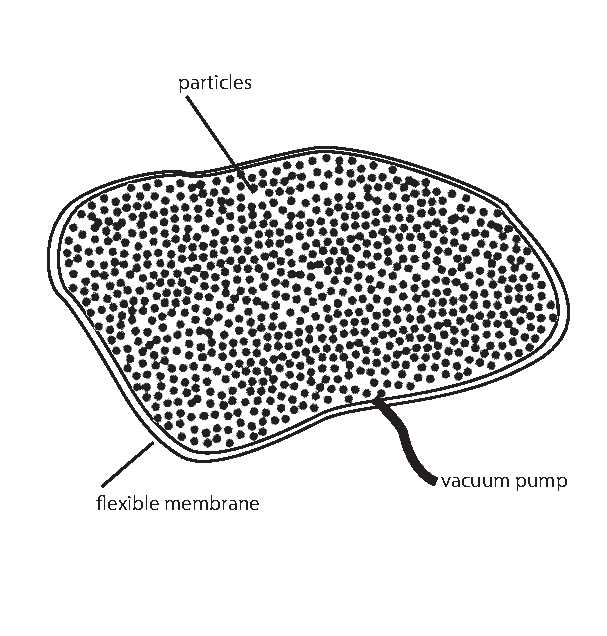
\includegraphics[width=\linewidth]{figures/jamming/basic_jamming}
    \caption[The basic jamming approach.]
    {Illustrates the basic approach with a single jammable volume.}
    \label{fig:ch:jamming:approaches:basic}     
  \end{minipage}
  \hspace{0.02\textwidth}
  \begin{minipage}[t]{.44\textwidth}
    \centering
    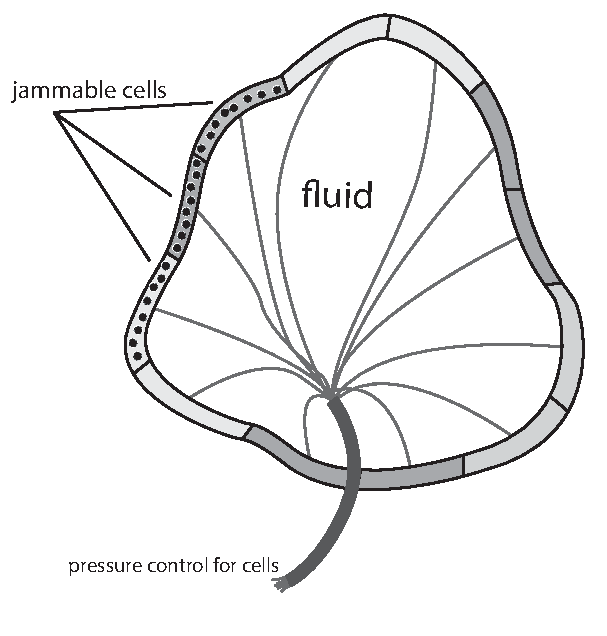
\includegraphics[width=\linewidth]{figures/jamming/cell_jamming}
    \caption[The cell-based jamming approach.]
    {Illustrates the cell-based approach where each cell functions as an independent jammable volume. An inner actuator can contract and expand to control pressure on the cell.}
    \label{fig:ch:jamming:approaches:cell}
  \end{minipage}%
\end{figure}

